\begin{center} \resizebox{0.95\textwidth}{!}{ 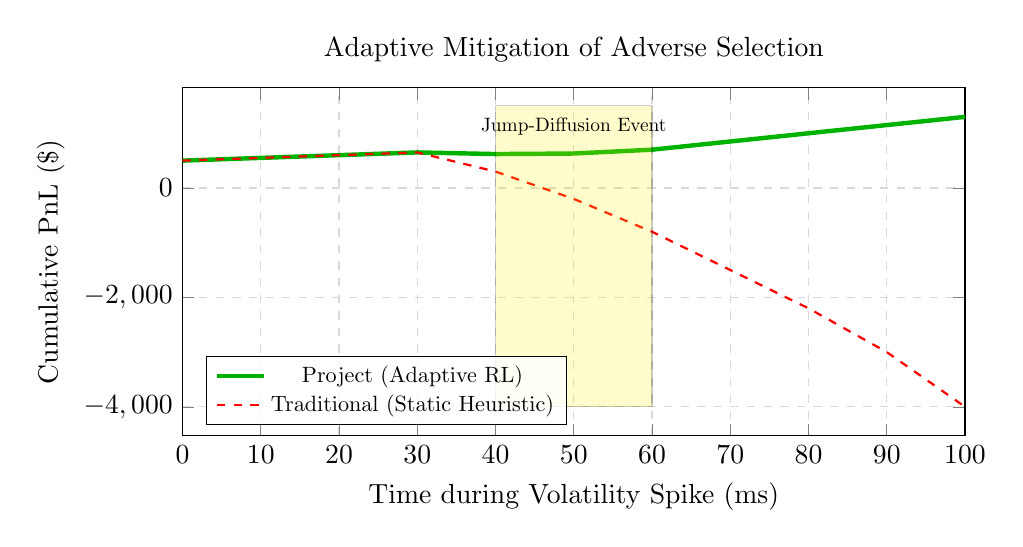
\begin{tikzpicture} \begin{axis}[ width=0.95\columnwidth, height=6cm, xlabel={Time during Volatility Spike (ms)}, ylabel={Cumulative PnL ($\$$)}, xmin=0, xmax=100, grid=major, grid style={dashed, gray!30}, title={Adaptive Mitigation of Adverse Selection}, legend pos=south west, legend style={nodes={scale=0.8, transform shape}, fill=white, fill opacity=0.8, draw opacity=1, text opacity=1}, y tick label style={/pgf/number format/fixed, /pgf/number format/1000 sep={,}}, scaled y ticks=false ] \addplot[color=green!70!black, ultra thick] coordinates  { (0, 500) (10, 550) (20, 600) (30, 650) (40, 620) (50, 630) (60, 700) (70, 850) (80, 1000) (90, 1150) (100, 1300) }; \addlegendentry{Project (Adaptive RL)} \addplot[color=red, thick, dashed] coordinates  { (0, 500) (10, 550) (20, 600) (30, 650) (40, 300) (50, -200) (60, -800) (70, -1500) (80, -2200) (90, -3000) (100, -4000) }; \addlegendentry{Traditional (Static Heuristic)} \draw[fill=yellow, opacity=0.2] (axis cs: 40, -4000) rectangle (axis cs: 60, 1500); \node[anchor=north, scale=0.7] at (axis cs: 50, 1400) {Jump-Diffusion Event}; \end{axis} \end{tikzpicture} } \end{center}